\section{Arquitectura funcional final del sistema}

El resultado final del proyecto se materializa en una aplicación web desarrollada con \textbf{Flask}, concebida como herramienta educativa de simulación de inversión sobre datos históricos reales. La solución combina una capa de presentación basada en plantillas HTML renderizadas en servidor, una capa de lógica de aplicación en Python y una capa de persistencia orientada a soportar autenticación, historial y continuidad entre modos de uso.

Desde el punto de vista funcional, la aplicación se estructura alrededor de cuatro bloques principales: el acceso al sistema, el modo de práctica, el modo carrera y el modo horizonte. Sobre estos bloques se apoya una capa pedagógica adicional formada por la sección de aprendizaje, el \textit{readiness quiz} y el tutor de IA opcional asociado al informe final del modo carrera.

\subsection{Estructura general de la aplicación}

La arquitectura implementada mantiene una separación clara entre responsabilidades:

\begin{itemize}
    \item \textbf{Capa de presentación:} construida mediante plantillas \texttt{Jinja2}, hojas de estilo CSS personalizadas y componentes de interacción en JavaScript. Esta capa se encarga de la representación de pantallas, formularios, tablas y gráficos.
    \item \textbf{Capa de control:} desarrollada en Flask mediante rutas y \textit{blueprints}. Gestiona el enrutamiento HTTP, la validación de entradas, la composición de respuestas HTML y JSON y la coordinación entre usuario, sesión y servicios de dominio.
    \item \textbf{Capa de lógica de negocio:} concentra la simulación financiera, la gestión del modo carrera, la generación de métricas comparativas, la construcción del informe final y la preparación de escenarios experimentales en el modo horizonte.
    \item \textbf{Capa de persistencia y servicios:} integra el acceso a PostgreSQL en Render, la autenticación por correo electrónico y contraseña, el historial de análisis, la persistencia de sesiones del modo carrera y los servicios auxiliares del sistema.
\end{itemize}

La estructura final no responde ya a un prototipo anónimo y efímero, sino a una solución web modular con diferenciación de usuarios, persistencia selectiva y validación progresiva del aprendizaje.

\begin{figure}[h]
    \centering
    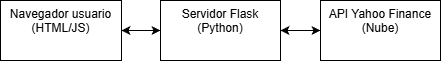
\includegraphics[width=0.84\textwidth]{figs/arquitectura.png}
    \caption{Arquitectura de alto nivel de la aplicación en su estado final.}
    \label{fig:arquitectura_final}
\end{figure}

\subsection{Módulos principales}

Los módulos funcionales que articulan la aplicación son los siguientes:

\begin{itemize}
    \item \textbf{Inicio y acceso al sistema:} ofrece entrada mediante autenticación, registro o modo invitado.
    \item \textbf{Aprender:} presenta contenidos introductorios, explica la lógica del simulador y sirve de antesala pedagógica al cuestionario de preparación.
    \item \textbf{Readiness quiz:} evalúa conocimientos mínimos y actúa como mecanismo de desbloqueo del modo carrera.
    \item \textbf{Modo Práctica:} permite realizar análisis puntuales de empresas y comparar resultados con referencias de mercado.
    \item \textbf{Modo Carrera:} organiza una experiencia de simulación por turnos, con persistencia, informe final y continuidad pedagógica.
    \item \textbf{Modo Horizonte:} genera una proyección experimental basada en patrones históricos, con advertencias explícitas y sin carácter predictivo.
    \item \textbf{Tutor IA:} aporta una capa opcional de análisis educativo sobre el informe final del modo carrera.
\end{itemize}

\section{Gestión de usuarios y persistencia}

Una de las transformaciones más relevantes del proyecto durante su evolución fue el paso desde una experiencia esencialmente anónima a un modelo mixto que distingue entre \textbf{usuario registrado} y \textbf{usuario invitado}. Esta distinción afecta de manera directa a la persistencia del historial, la continuidad entre sesiones y el acceso a determinadas funcionalidades.

\subsection{Autenticación por correo electrónico}

Se implementó un flujo de autenticación basado en correo electrónico y contraseña. La aplicación permite registrar cuentas, iniciar sesión, cerrar sesión y mantener el estado autenticado mediante la sesión de Flask. El almacenamiento de credenciales se realiza de forma segura mediante funciones de \textit{hash} de contraseña, evitando el almacenamiento en texto plano.

Este modelo de acceso resuelve una limitación importante de las primeras versiones del sistema, en las que el uso sin identidad impedía conservar el historial y dificultaba la continuidad real de aprendizaje entre distintas visitas.

\begin{figure}[h]
    \centering
    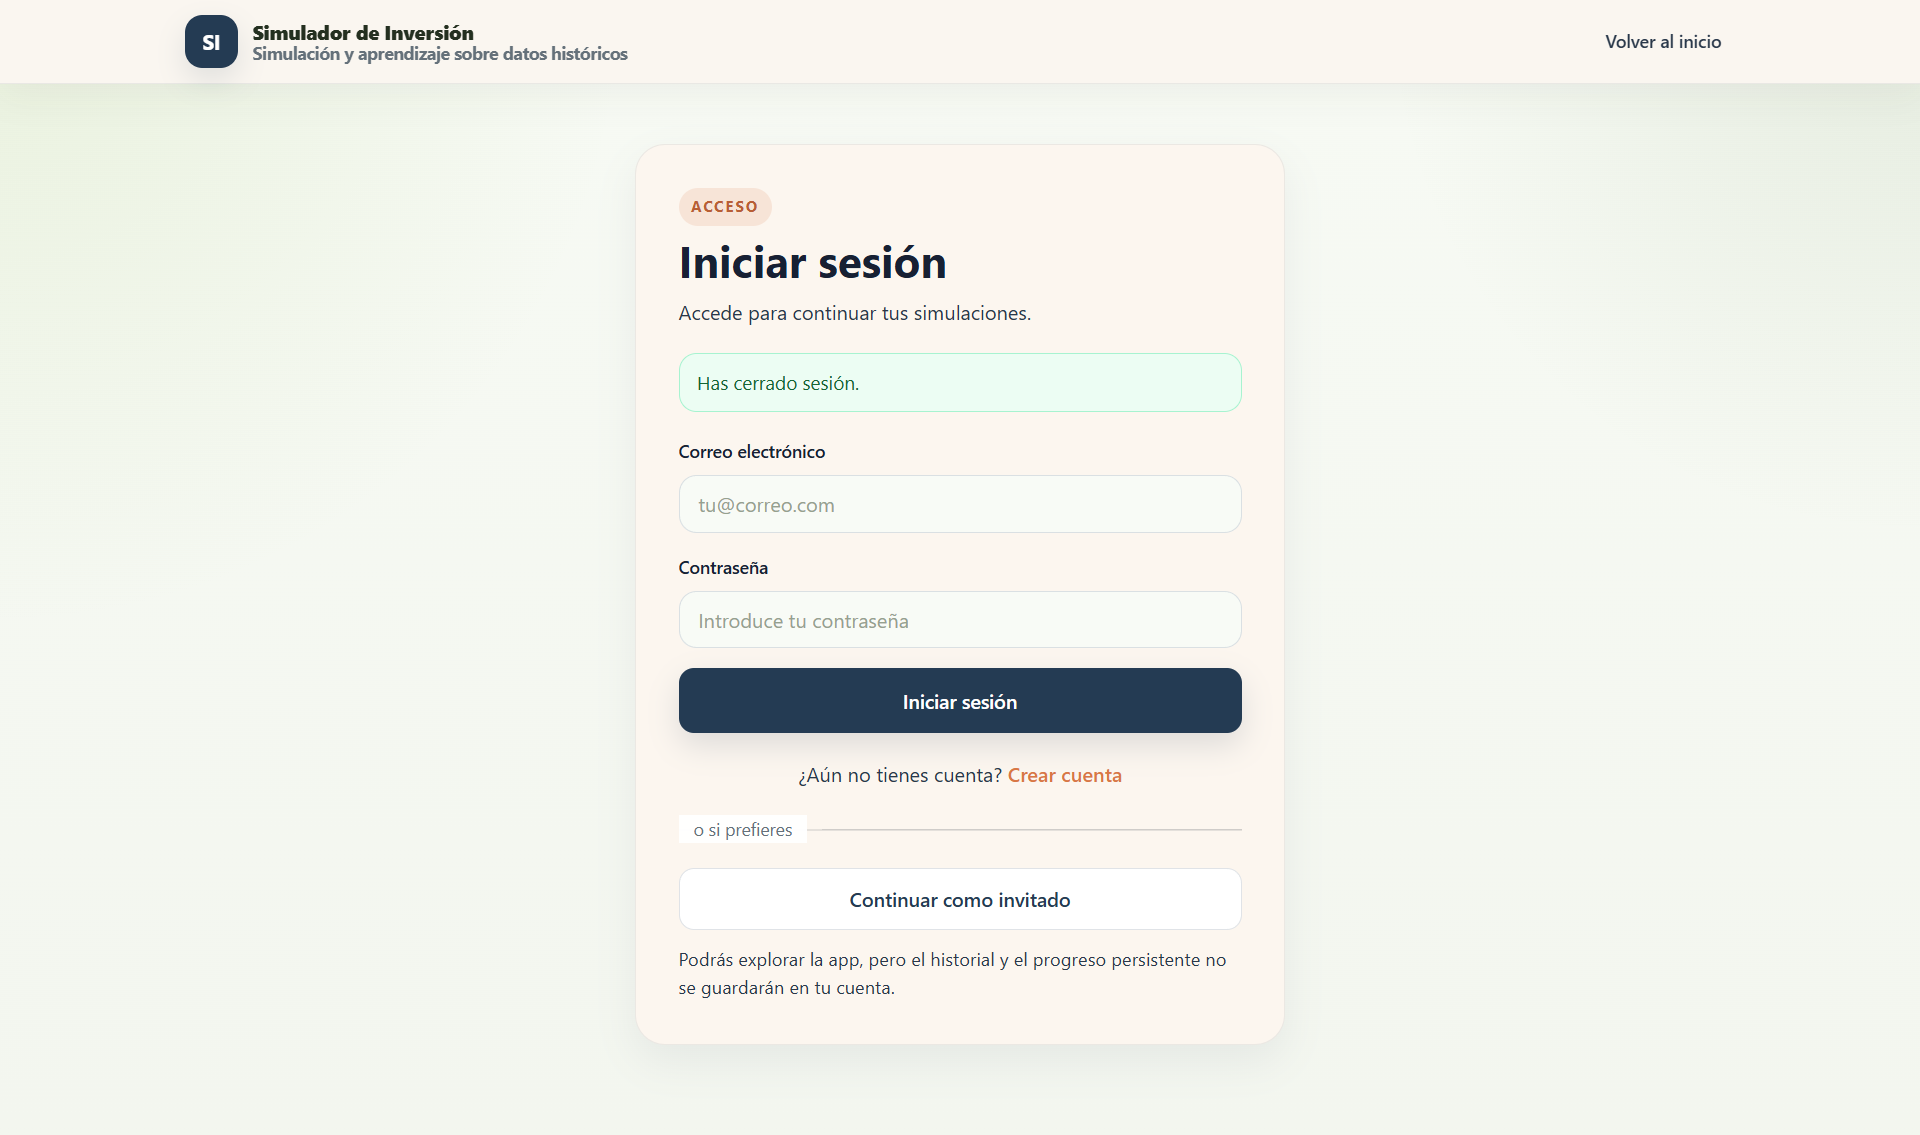
\includegraphics[width=0.78\textwidth]{figs/login_final.png}
    \caption{Pantalla de acceso tras la integración de autenticación por correo y el rediseño visual final.}
    \label{fig:login_final}
\end{figure}

\subsection{Usuario autenticado frente a usuario invitado}

El sistema final diferencia dos formas principales de uso:

\begin{itemize}
    \item \textbf{Usuario autenticado:} dispone de historial persistente, continuidad de progreso, conservación del aprobado del cuestionario y acceso estable a las sesiones del modo carrera.
    \item \textbf{Usuario invitado:} puede explorar la aplicación sin crear cuenta, pero no conserva historial persistente entre sesiones y su uso queda acotado a una experiencia más limitada.
\end{itemize}

Esta separación resultó especialmente importante desde el punto de vista de producto, ya que permitió mantener una barrera de entrada baja sin renunciar a una capa real de continuidad para el usuario que decide implicarse más en la simulación.

\subsection{Persistencia con PostgreSQL en Render}

La persistencia final del sistema se apoya en una base de datos \textbf{PostgreSQL} desplegada en Render. Sobre ella se almacenan los elementos críticos de continuidad del sistema: usuarios, historial de análisis, resultados del \textit{readiness quiz} y sesiones persistentes del modo carrera.

La capa de acceso se implementó mediante \textbf{Peewee}, lo que permitió mantener un modelo de datos ligero pero suficiente para el alcance del TFG. La decisión de utilizar PostgreSQL en producción sustituyó las limitaciones de un enfoque puramente efímero y permitió validar el producto en condiciones más cercanas a un despliegue real.

Durante la fase final del proyecto se produjo además la expiración de una base de datos previa en Render. La creación de una nueva instancia y su integración satisfactoria en el sistema formó parte de la estabilización final del producto, validándose posteriormente el flujo de autenticación, la persistencia del historial y la navegación con usuario real.

\subsection{Historial y continuidad funcional}

El historial persistente quedó reservado al usuario autenticado. Esta decisión se mantuvo de forma coherente en todo el sistema:

\begin{itemize}
    \item los análisis del modo práctica se asocian al usuario autenticado;
    \item las sesiones y turnos del modo carrera pueden recuperarse en visitas posteriores;
    \item el resultado del cuestionario de preparación puede conservarse en la cuenta;
    \item el modo invitado mantiene una experiencia funcional, pero sin promesa de persistencia estable.
\end{itemize}

\section{Flujo de acceso y progresión educativa}

La aplicación no se diseñó únicamente como una herramienta de consulta financiera, sino como un entorno de aprendizaje progresivo. Por ello, la navegación final se articula alrededor de una secuencia de acceso, comprensión y simulación.

\subsection{Inicio, registro y login}

La página principal resume el sistema, sus modos de uso y las vías de acceso disponibles. Desde ella se puede continuar mediante registro, inicio de sesión o uso como invitado, dependiendo del perfil de usuario.

\begin{figure}[h]
    \centering
    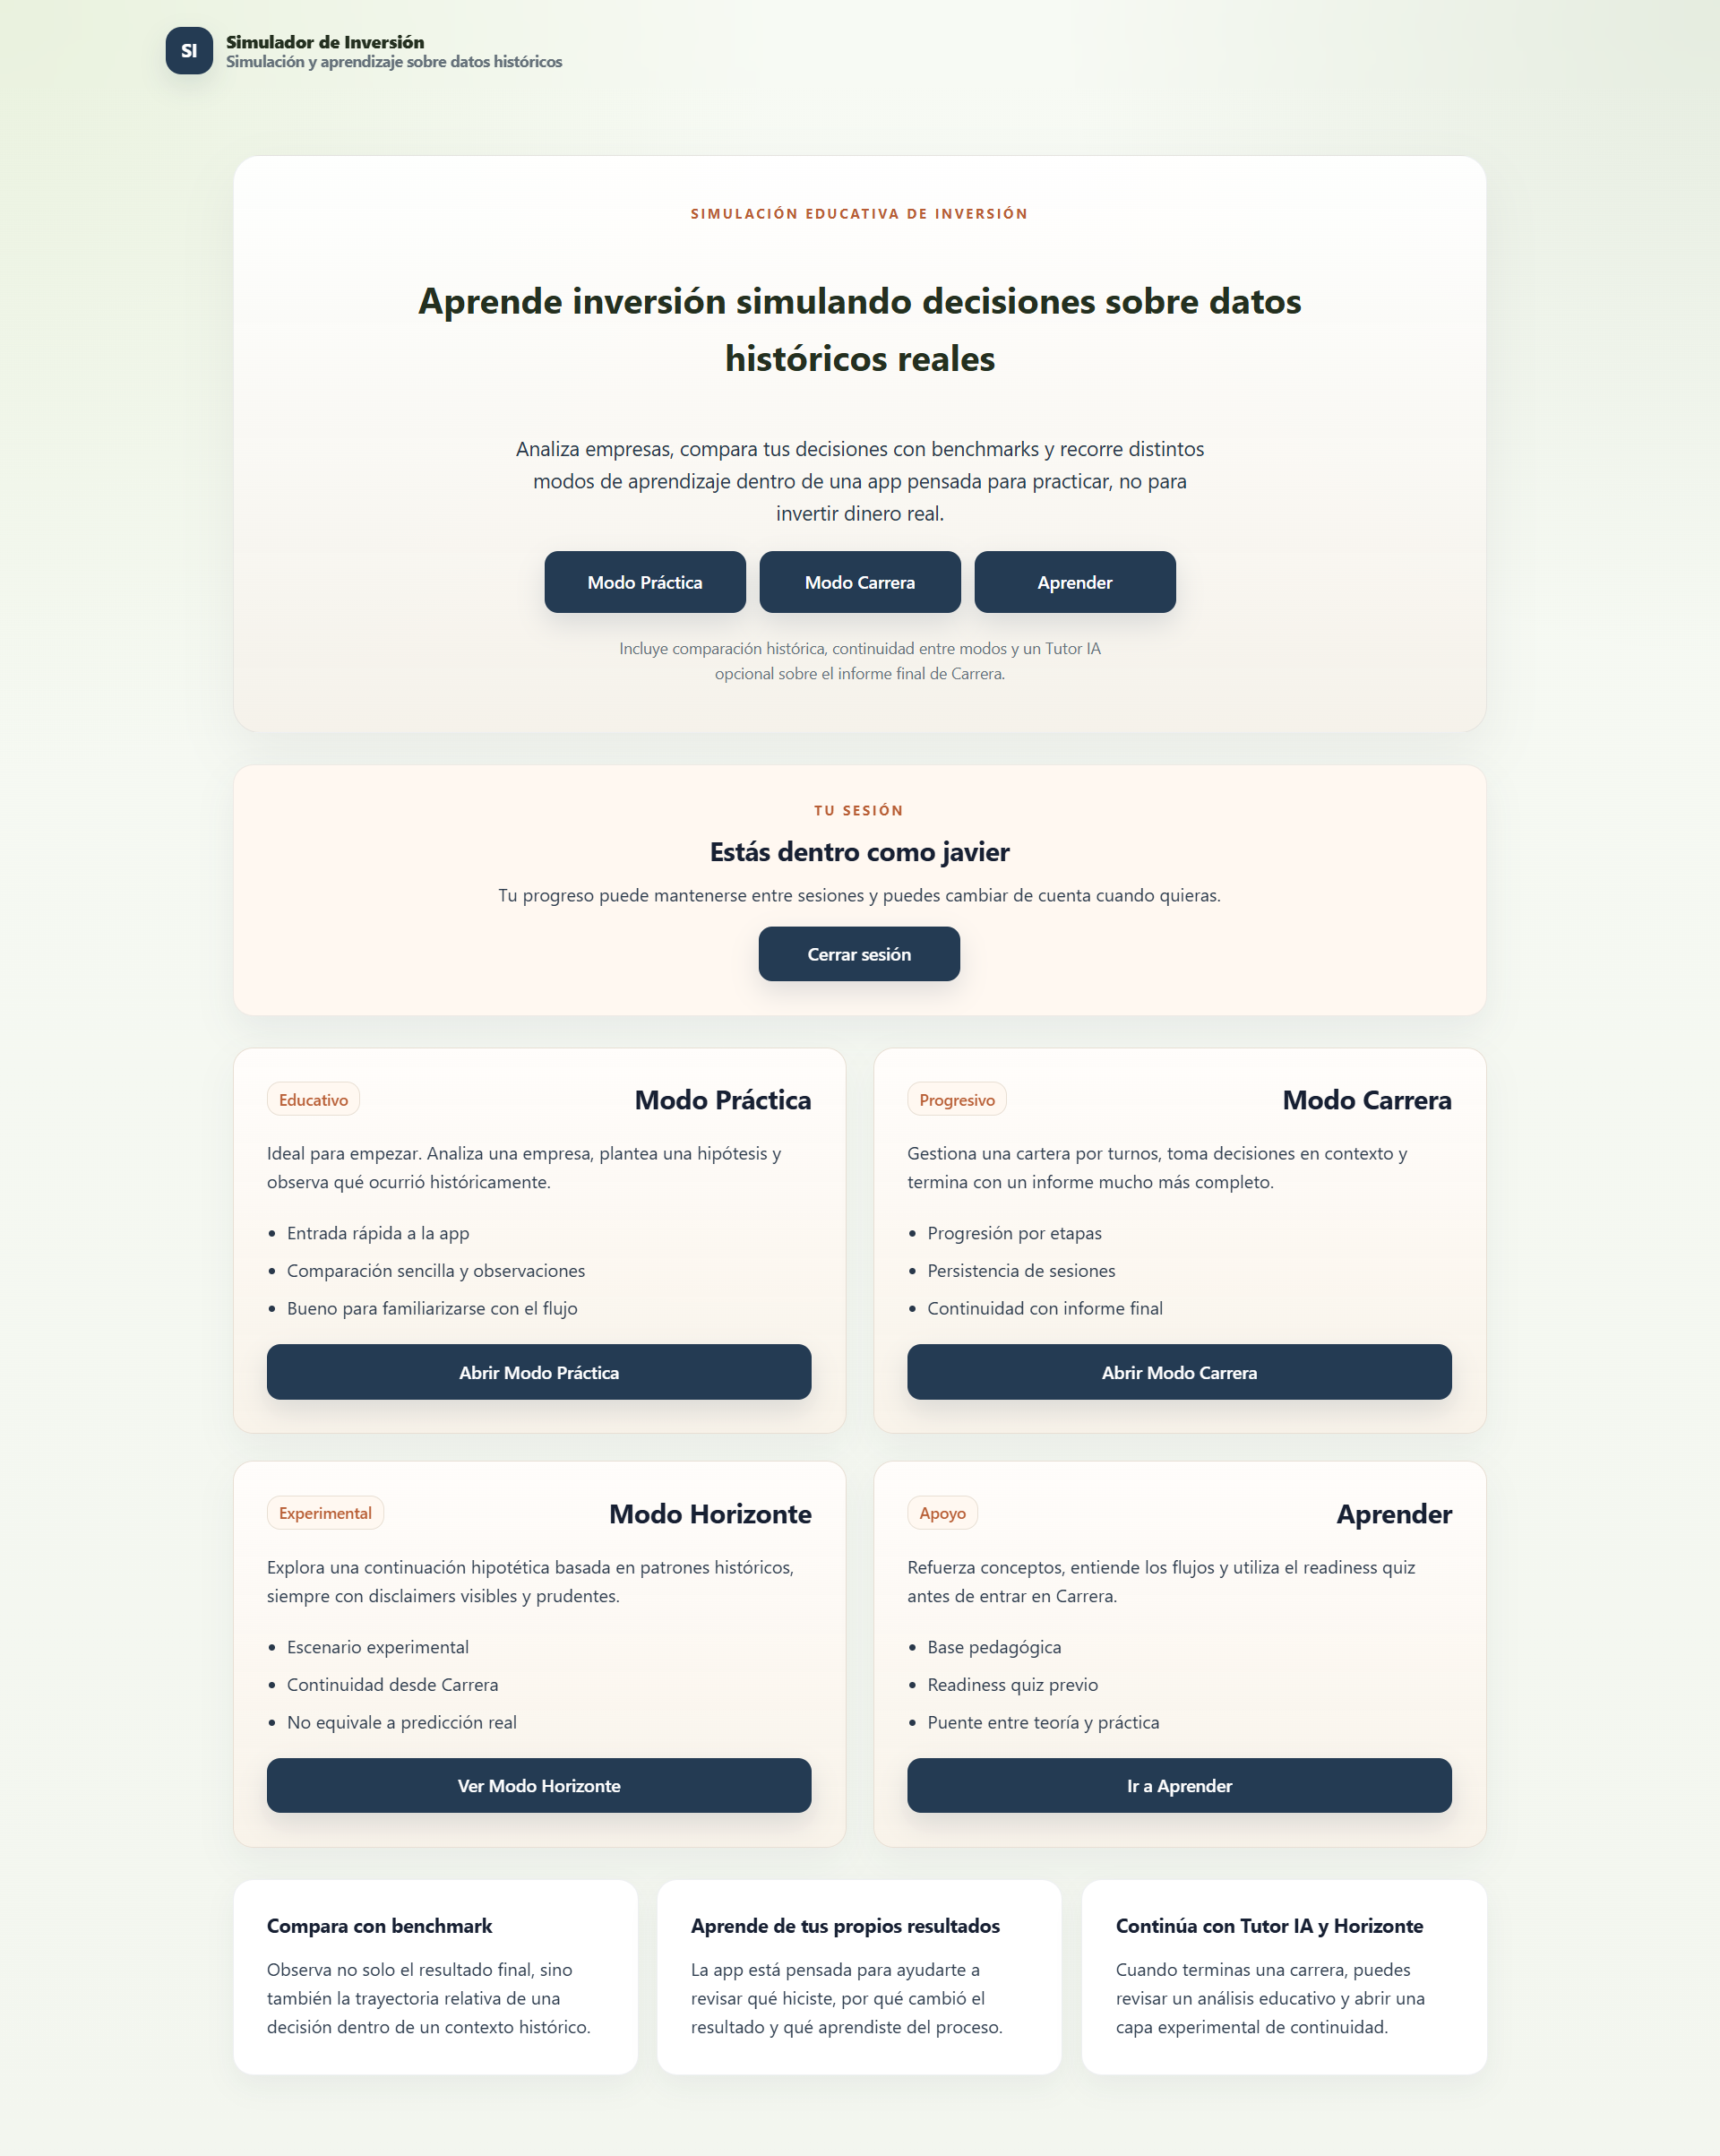
\includegraphics[width=0.82\textwidth]{figs/home_final.png}
    \caption{Pantalla principal final del sistema tras la consolidación del rediseño frontend.}
    \label{fig:home_final}
\end{figure}

La combinación entre identidad visual renovada y claridad de acceso ayudó a convertir la página de inicio en un punto de entrada coherente con el resto del producto.

\subsection{Aprender y readiness quiz}

La sección \textit{Aprender} cumple una doble función. Por una parte, introduce conceptos básicos y contextualiza el uso del simulador; por otra, actúa como soporte previo al \textit{readiness quiz}, concebido como mecanismo de desbloqueo progresivo del modo carrera.

Este cuestionario evita que el acceso al modo más complejo de la aplicación se produzca sin una base mínima de comprensión, reforzando el carácter pedagógico del sistema.

\begin{figure}[h]
    \centering
    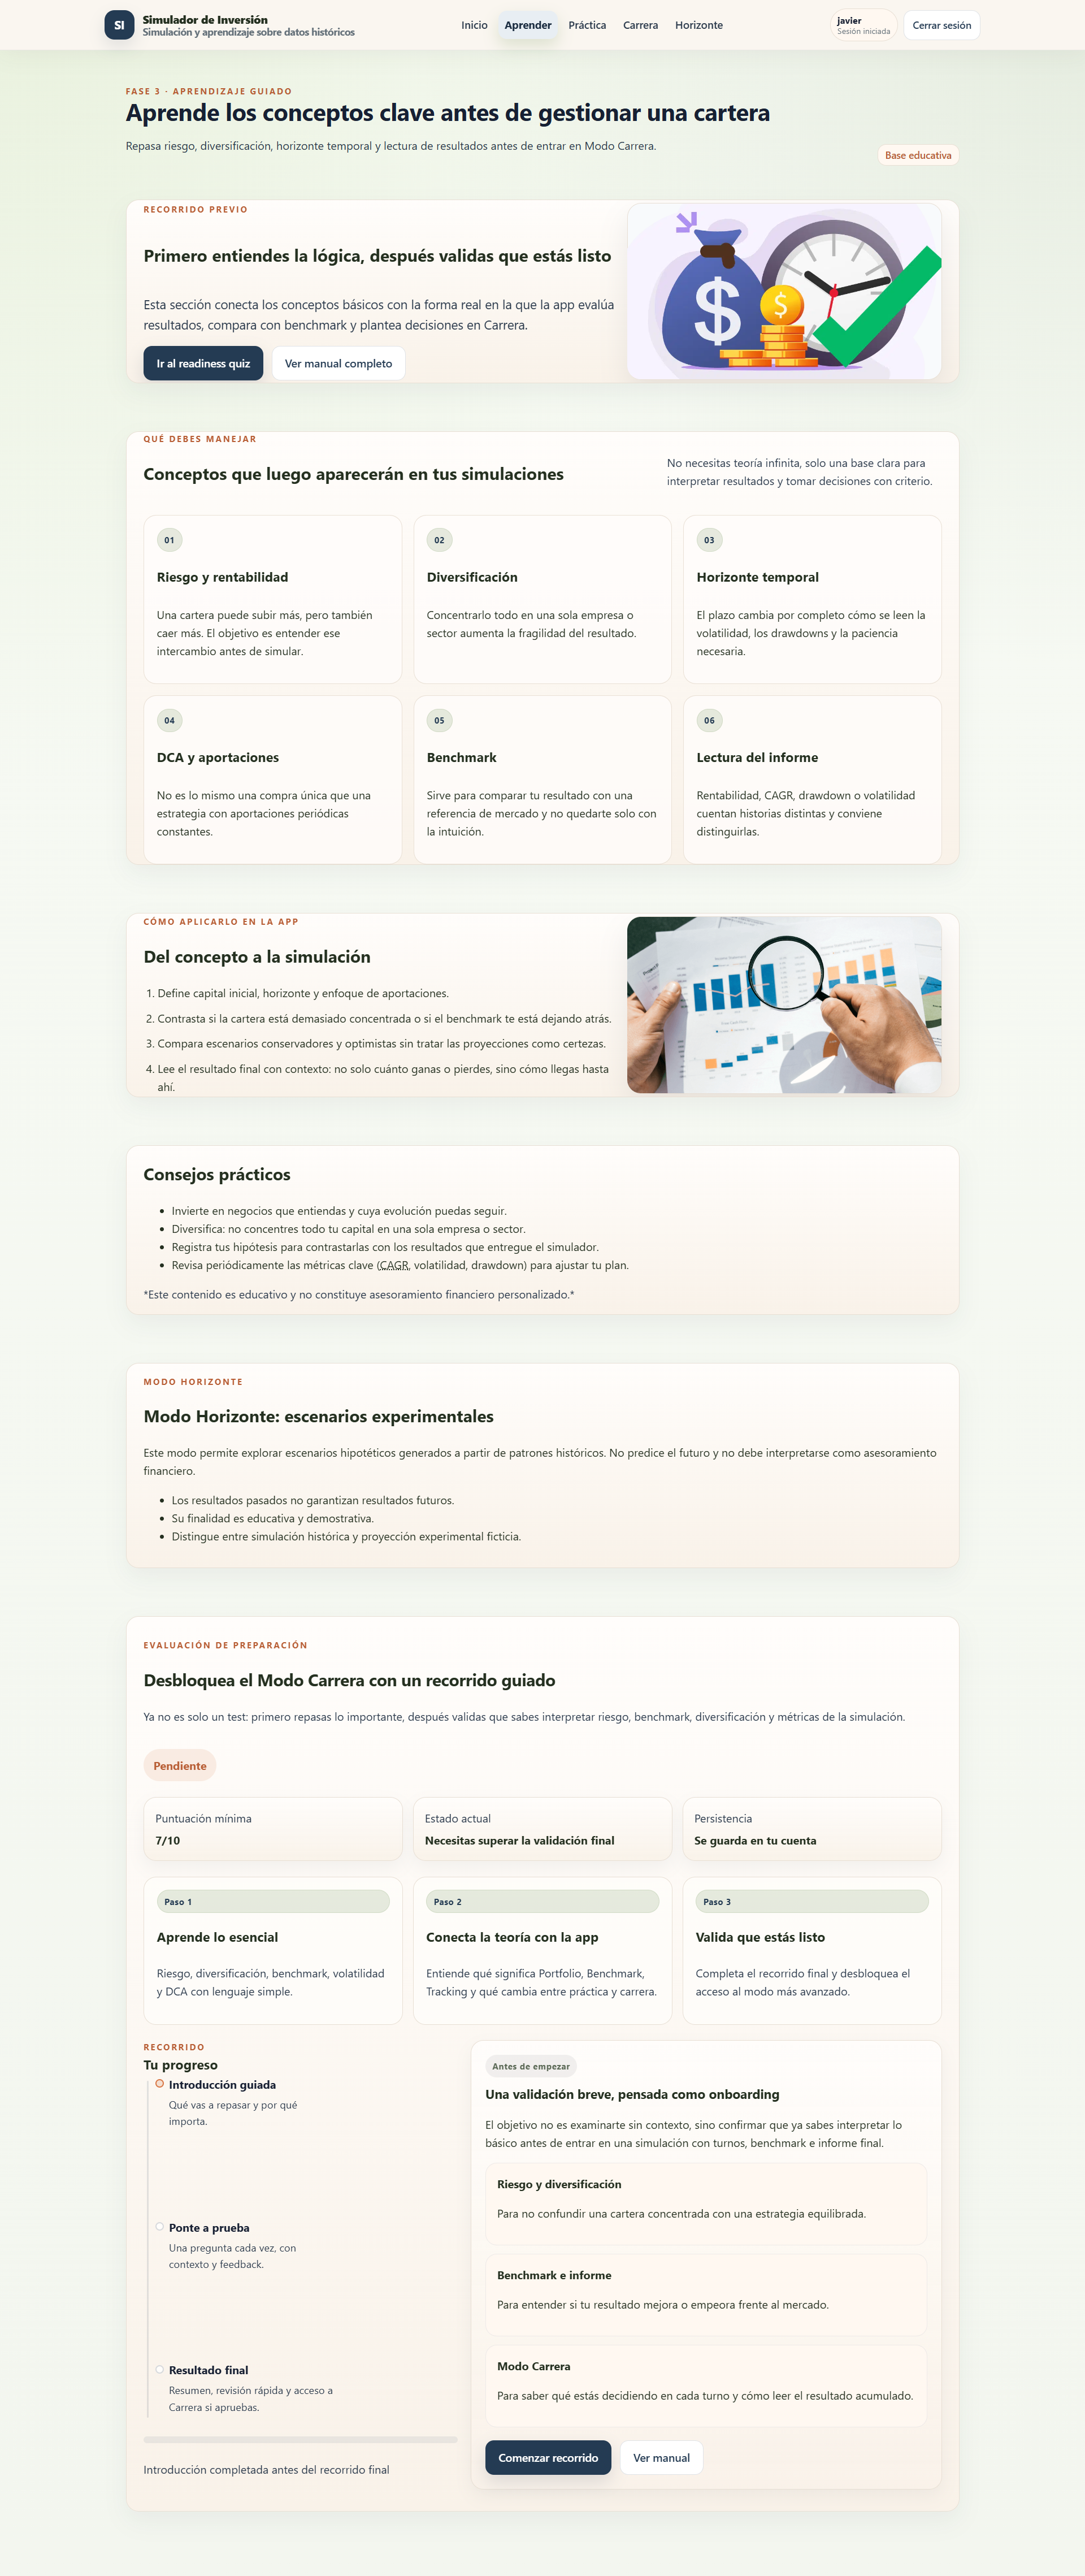
\includegraphics[width=0.8\textwidth]{figs/aprender_final.png}
    \caption{Pantalla \textit{Aprender}, diseñada como apoyo pedagógico al cuestionario de preparación y al acceso progresivo al modo carrera.}
    \label{fig:aprender_final}
\end{figure}

\subsection{Desbloqueo progresivo del modo carrera}

El modo carrera se mantuvo como bloque funcional diferenciado y de mayor exigencia. Su desbloqueo condicionado por el cuestionario permitió reforzar la coherencia entre teoría y práctica, y ofreció una transición más razonable entre una exploración inicial y una experiencia de simulación prolongada.

\section{Módulos principales del sistema}

\subsection{Modo Práctica o Nuevo análisis}

El modo práctica constituye la puerta de entrada funcional más directa al sistema. Permite seleccionar un activo, configurar parámetros de análisis y obtener una visualización histórica junto con métricas comparativas. Durante el desarrollo final se mantuvo intacta la lógica de cálculo, pero se reorganizó la experiencia como un flujo guiado con pasos más legibles y consistentes.

\begin{figure}[h]
    \centering
    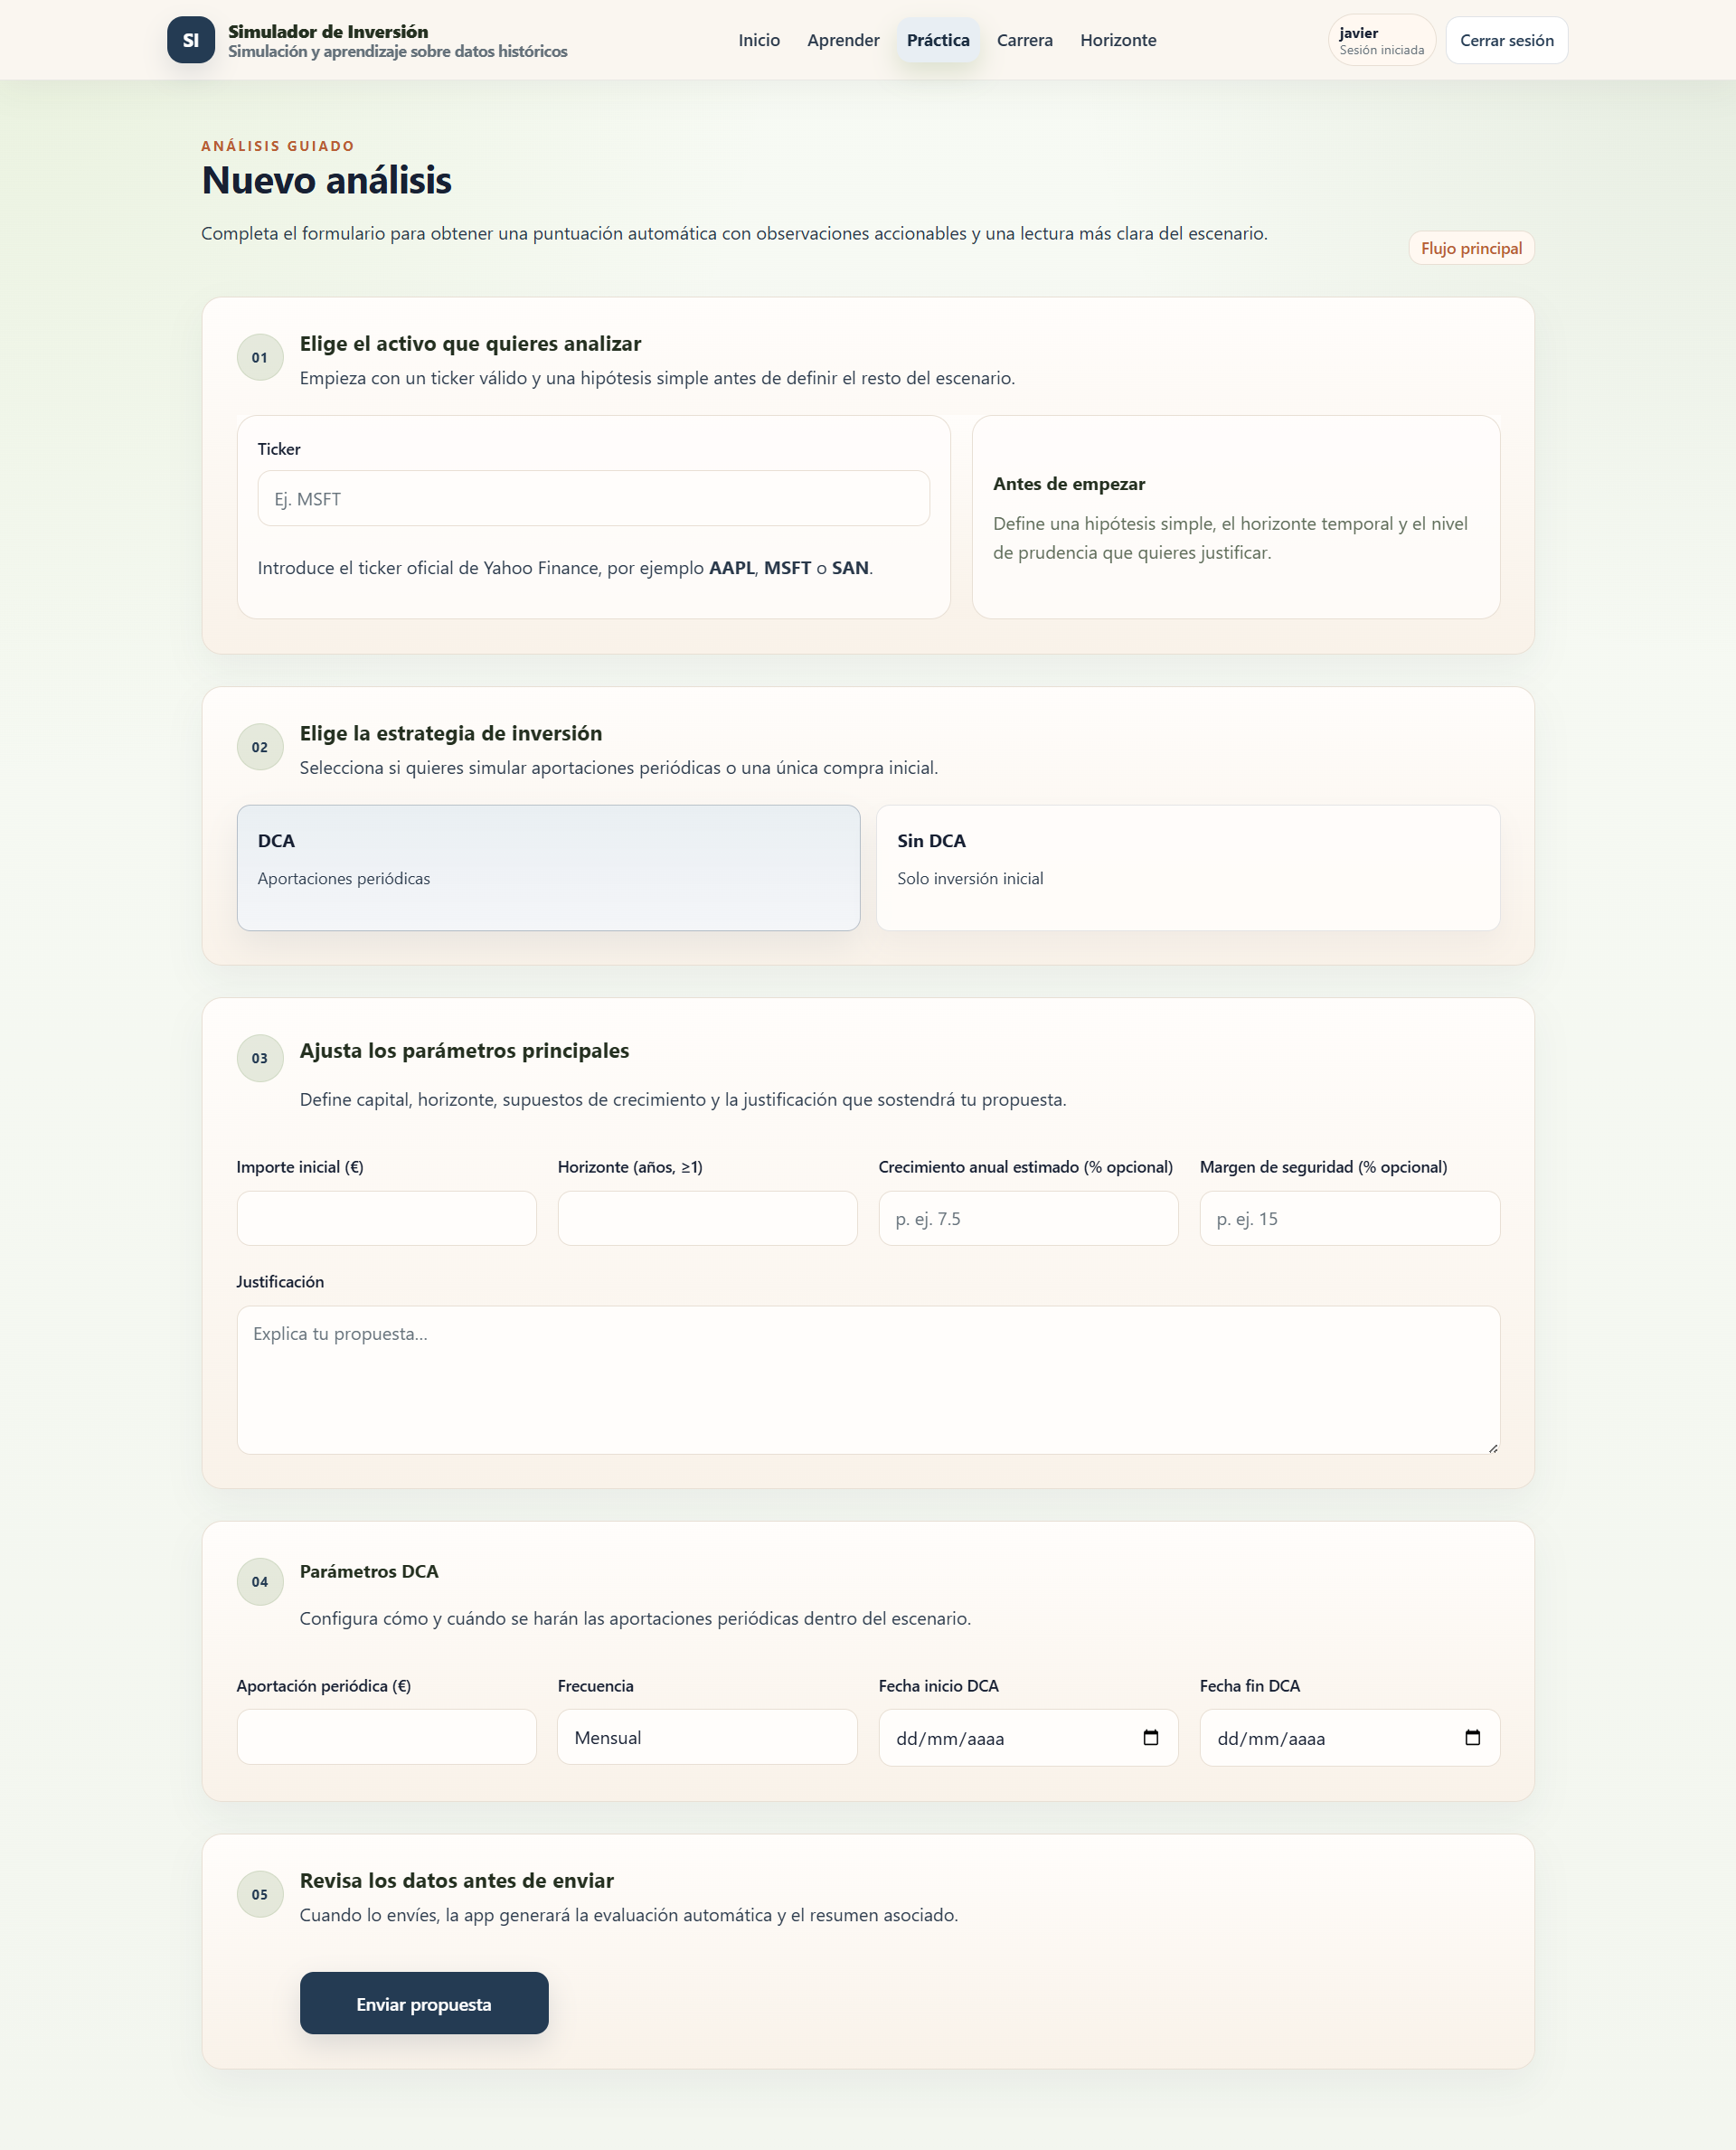
\includegraphics[width=0.8\textwidth]{figs/practica_final.png}
    \caption{Modo práctica rediseñado como flujo guiado de análisis sin alterar la lógica funcional del simulador.}
    \label{fig:practica_final}
\end{figure}

Este modo cumple una función clave: familiariza al usuario con el lenguaje de la aplicación antes de avanzar hacia dinámicas más complejas.

\subsection{Modo Carrera}

El modo carrera organiza una simulación por turnos en la que el usuario configura una sesión, ajusta su cartera a lo largo del tiempo y recibe un informe final. A nivel técnico, este módulo fue uno de los más exigentes del proyecto, ya que combinó persistencia, generación de eventos, cálculos comparativos, continuidad temporal y tratamiento visual de estados muy diversos.

La evolución del sistema llevó este modo desde una versión inicial funcional pero limitada hasta una experiencia más madura, con mejor jerarquía visual, persistencia profunda y recuperación estable de sesiones guardadas.

\begin{figure}[h]
    \centering
    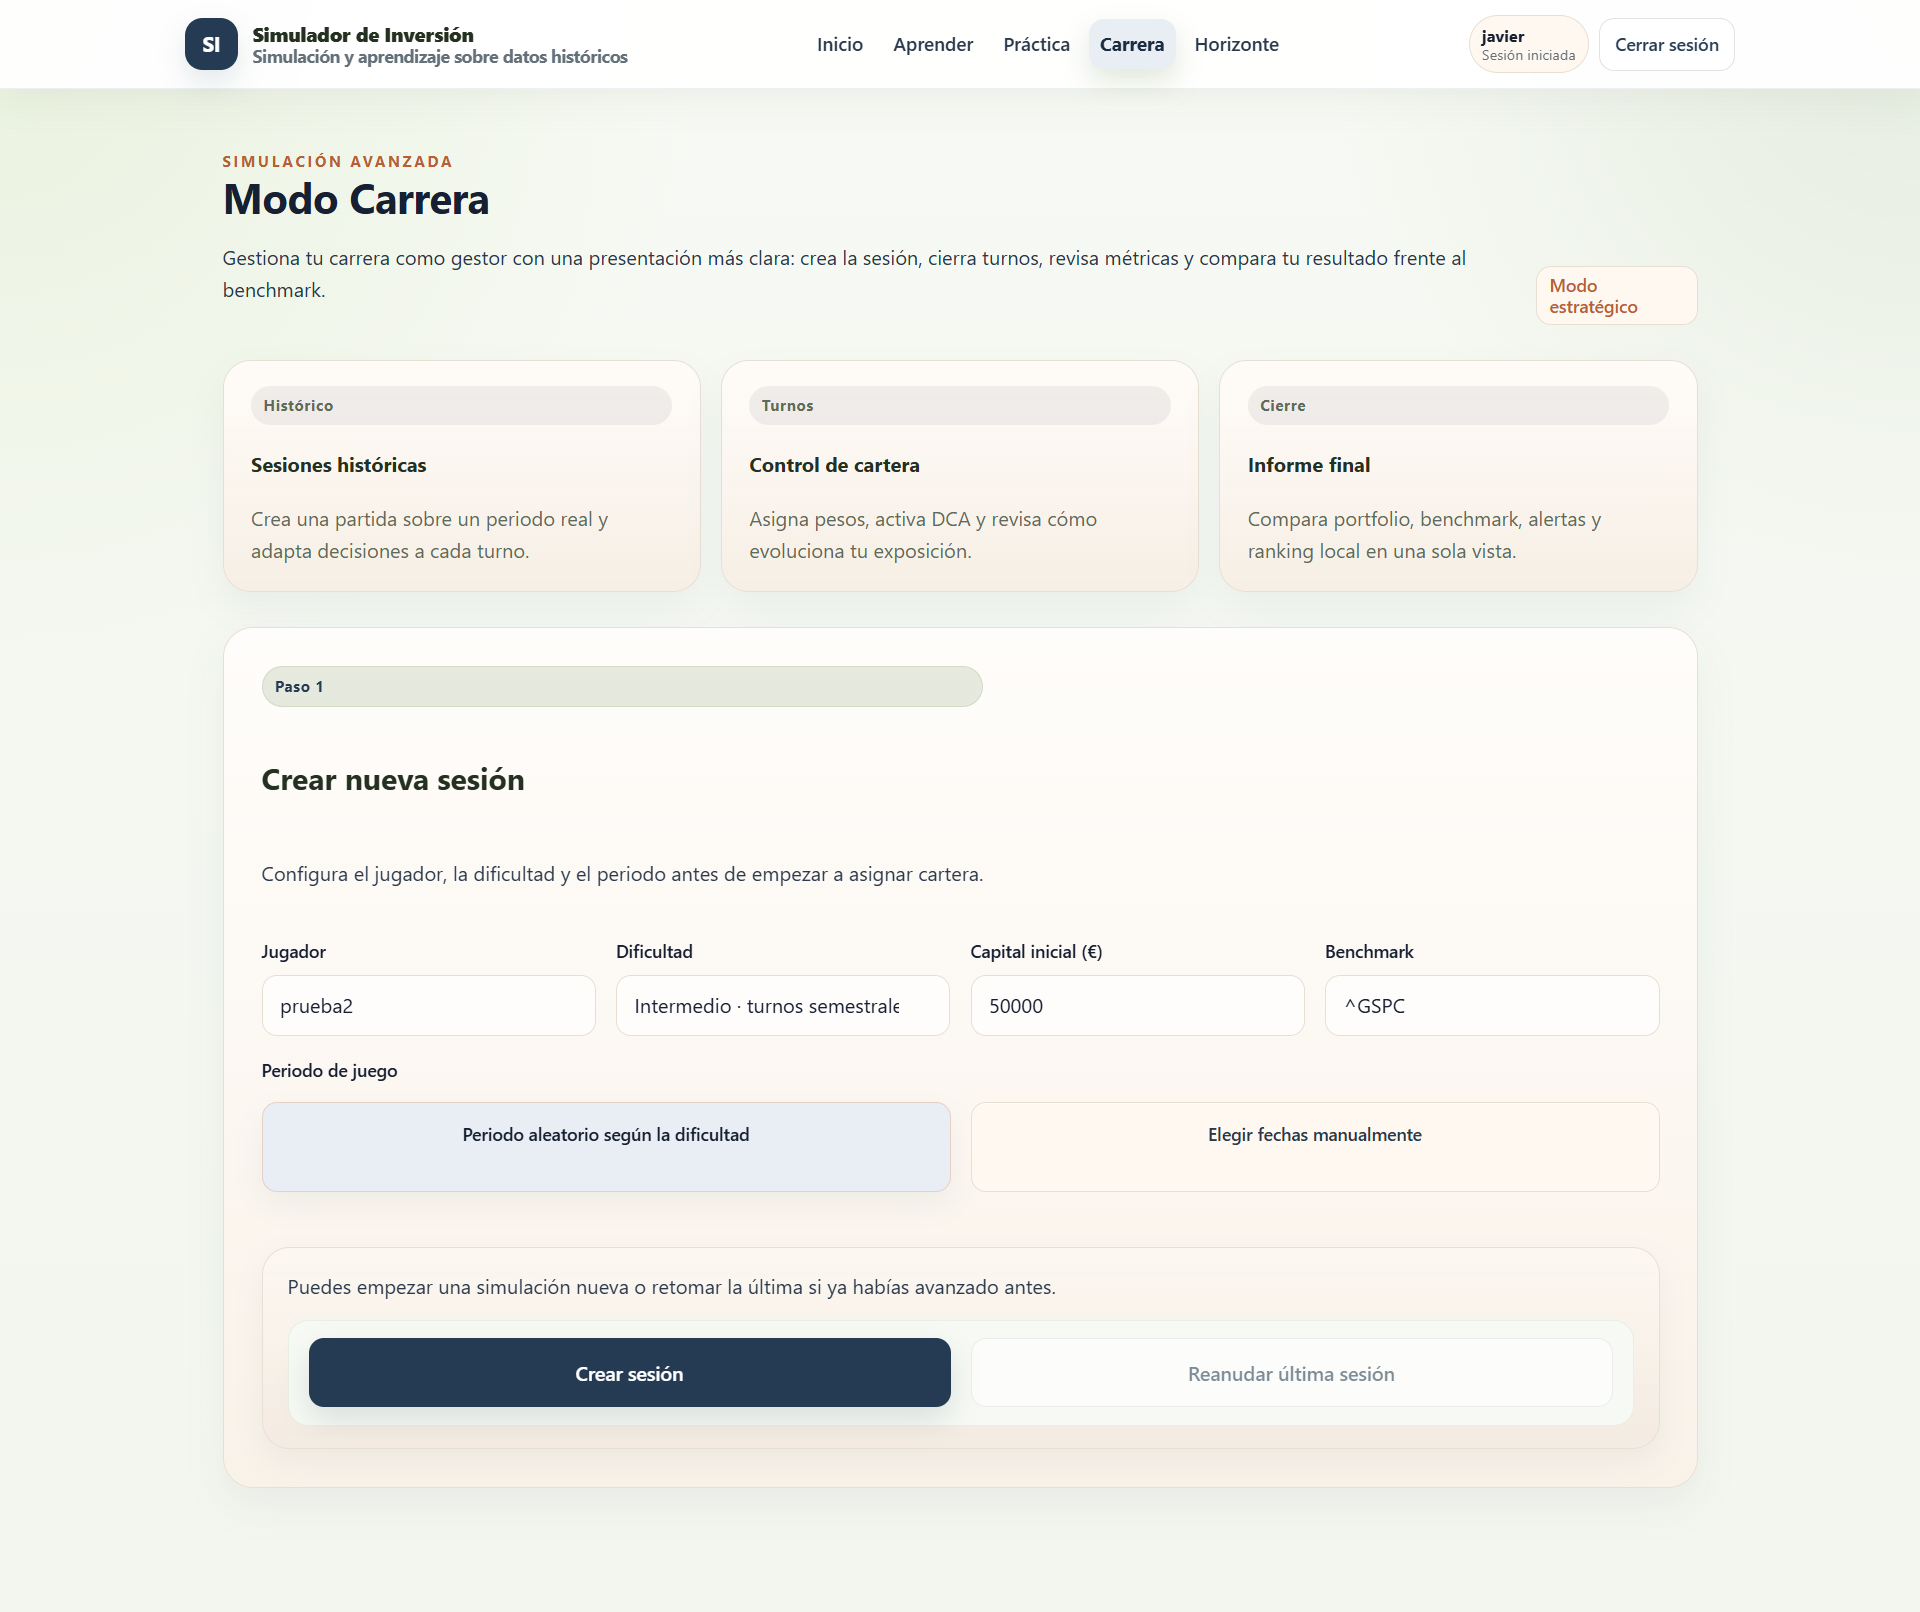
\includegraphics[width=0.82\textwidth]{figs/carrera_setup_final.png}
    \caption{Pantalla de configuración del modo carrera tras su rediseño visual y estabilización funcional.}
    \label{fig:carrera_setup_final}
\end{figure}

\subsection{Modo Horizonte}

El modo horizonte se incorporó como extensión experimental del ecosistema de simulación. Su finalidad no es predecir el mercado, sino construir un escenario hipotético a partir de patrones históricos. Por ello, se integró con advertencias explícitas, mensajes prudentes y una jerarquía visual que subraya su naturaleza educativa y no predictiva.

Este módulo también se diseñó para poder continuar desde el contexto final del modo carrera, transportando la información necesaria para mantener continuidad conceptual entre ambos modos.

\begin{figure}[h]
    \centering
    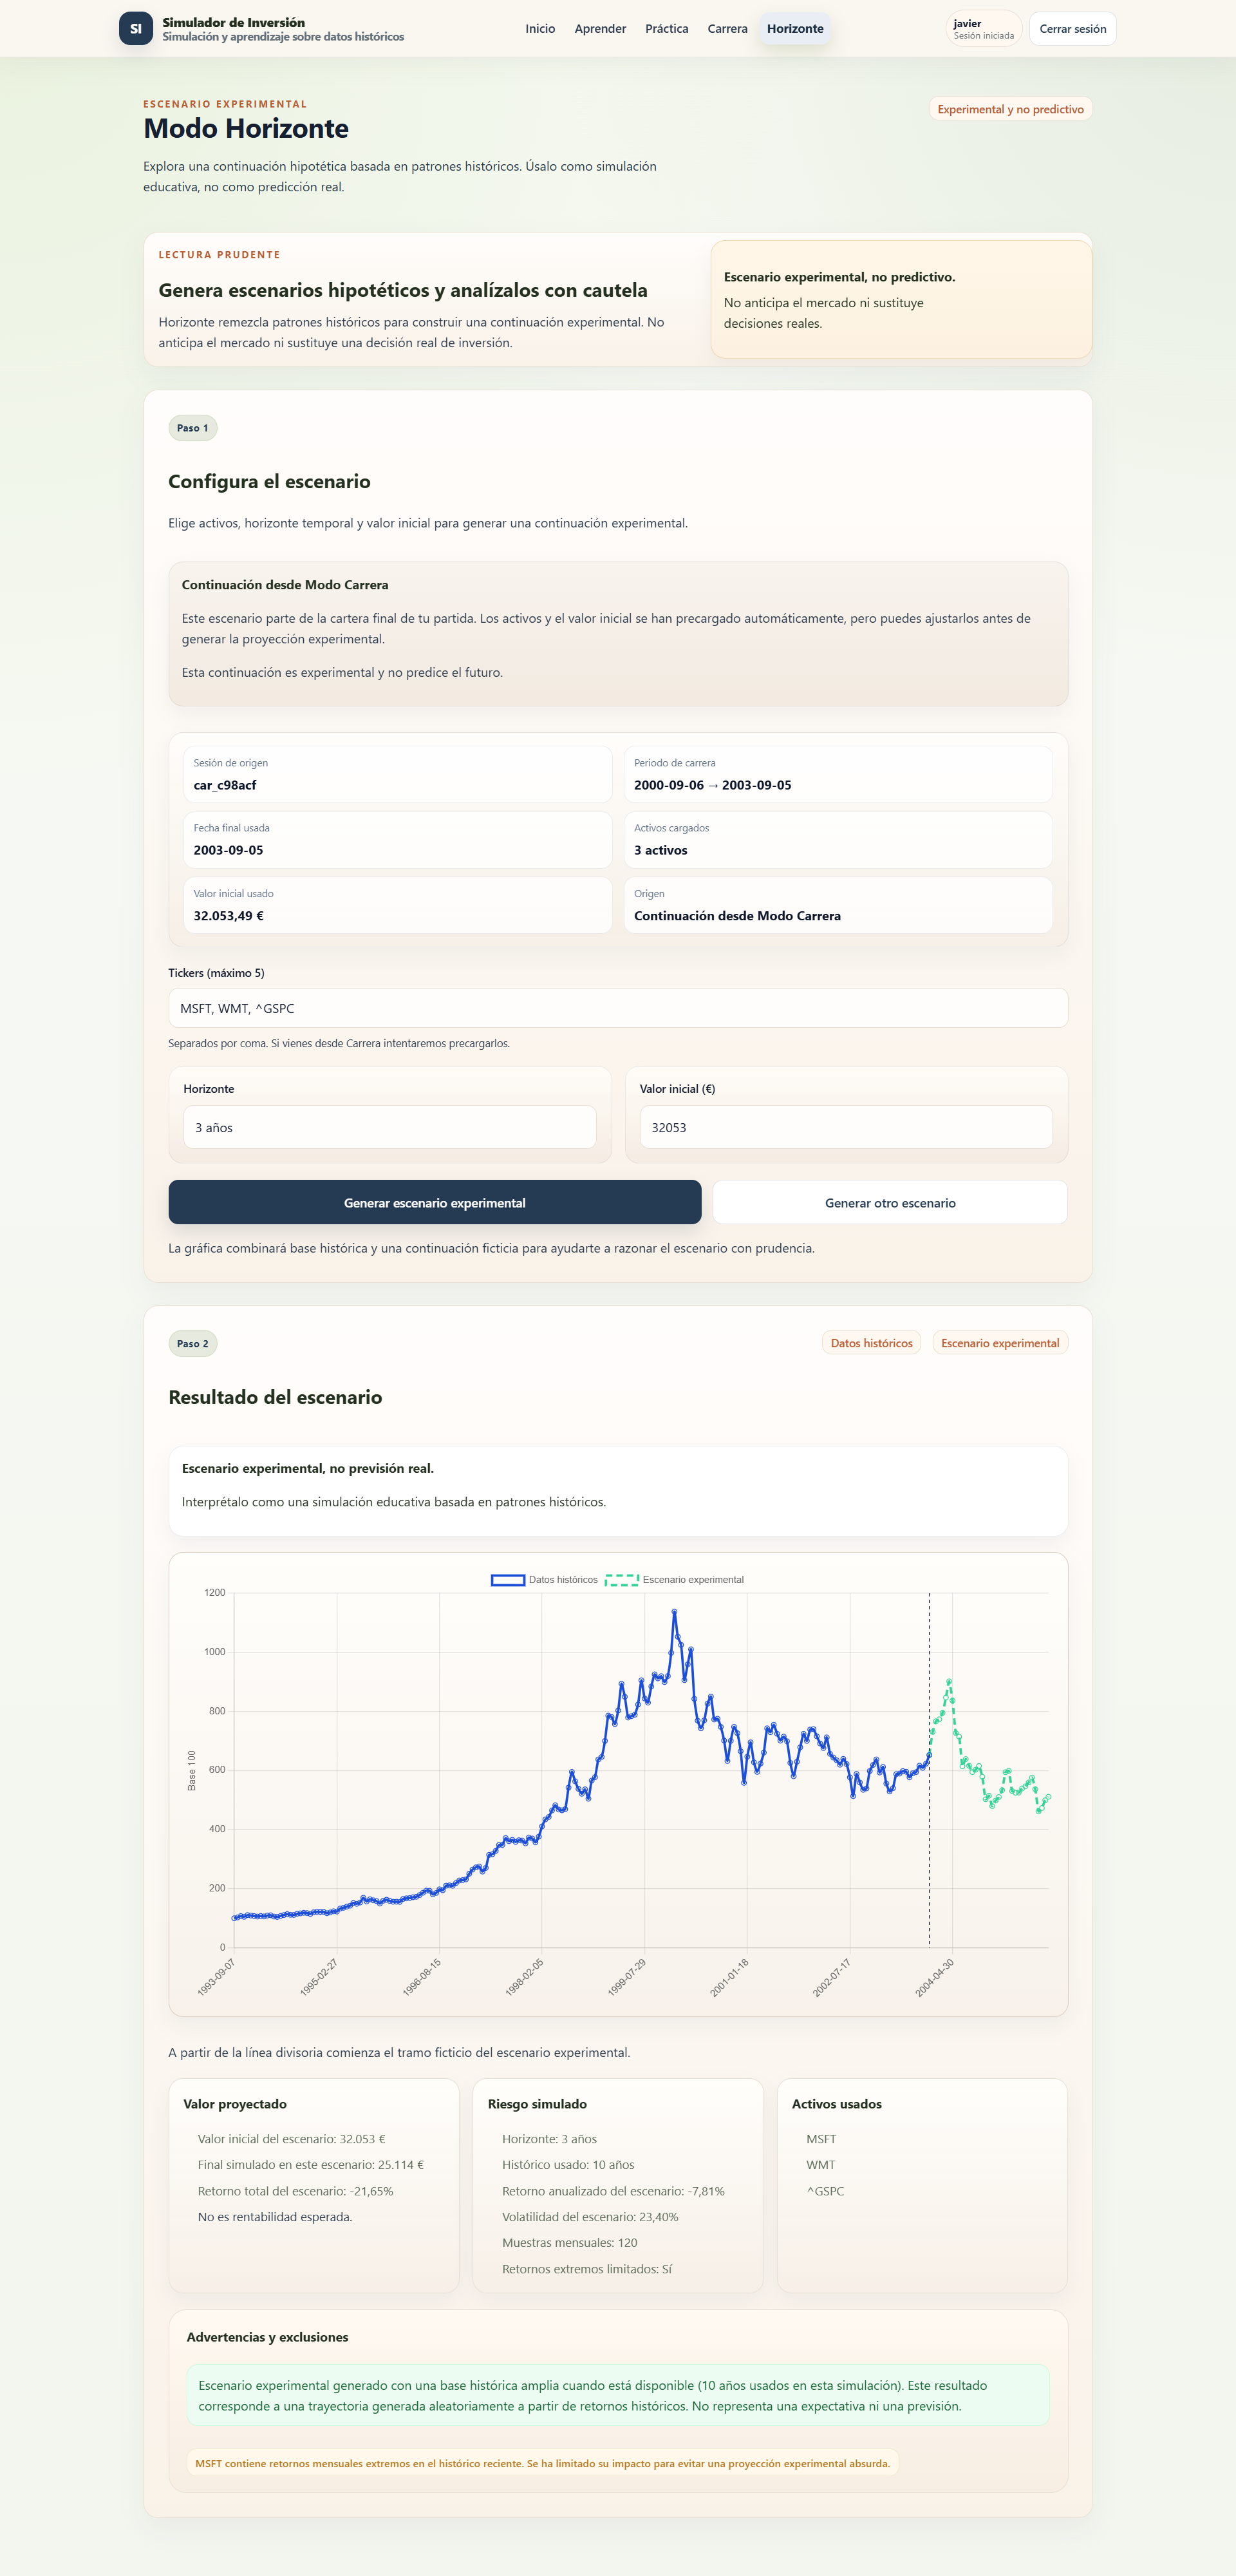
\includegraphics[width=0.82\textwidth]{figs/horizonte_final.png}
    \caption{Modo horizonte como herramienta experimental de proyección educativa, sin carácter predictivo ni función de asesoramiento financiero.}
    \label{fig:horizonte_final}
\end{figure}

\subsection{Tutor IA}

Sobre el informe final del modo carrera se añadió un tutor de IA opcional. Su función no consiste en recomendar compras o ventas reales, sino en analizar de forma educativa la simulación realizada y ayudar a interpretar decisiones, resultados y riesgos observados durante la partida.

La integración de este componente se diseñó bajo restricciones claras: uso opcional, dependencia de clave de entorno, control de tiempos de respuesta y salida prudente, evitando que el sistema pudiera interpretarse como una herramienta de asesoramiento financiero automático.

\section{Rediseño frontend por fases}

\subsection{Motivación del rediseño}

A medida que el proyecto fue creciendo en funcionalidades, la interfaz original empezó a mostrar síntomas claros de fragmentación: exceso de bloques heterogéneos, jerarquía visual débil, textos redundantes, formularios poco consistentes y pantallas que no siempre parecían pertenecer al mismo producto. Esto justificó la apertura de un rediseño visual por fases, realizado sin reescribir la lógica funcional ya estabilizada.

Los criterios de trabajo se centraron en mejorar la jerarquía visual, reducir texto innecesario, unificar botones y formularios, reforzar el comportamiento \textit{responsive} y clarificar la diferencia entre explicación pedagógica y herramienta operativa.

\subsection{Sistema visual base}

La primera fase del rediseño estableció un sistema visual común: paleta cromática, superficies, tipografía, botones, tarjetas, formularios, espaciado y comportamiento general de los estados principales. Esta base permitió que las fases posteriores pudieran trabajar sobre pantallas concretas sin abrir un rediseño arbitrario de cada módulo.

\subsection{Fases del rediseño}

La evolución del frontend se organizó en siete fases principales, resumidas en la Tabla~\ref{tab:rediseno_fases}.

\begin{table}[h]
\centering
\renewcommand{\arraystretch}{1.25}
\begin{tabular}{|p{0.1\textwidth}|p{0.28\textwidth}|p{0.25\textwidth}|p{0.25\textwidth}|}
\hline
\textbf{Fase} & \textbf{Pantallas / alcance} & \textbf{Objetivo principal} & \textbf{Resultado} \\ \hline
1 & Sistema visual base & Unificar tokens, superficies, tipografía y controles & Base estética coherente para el resto del producto \\ \hline
2 & Home, login, registro y navbar & Mejorar la primera impresión y la entrada al sistema & Acceso más claro y coherencia global inicial \\ \hline
3 & Aprender y readiness quiz & Reforzar la capa pedagógica y la progresión & Relación más clara entre teoría y simulación \\ \hline
4 & Modo práctica / nuevo análisis & Convertir el análisis en flujo guiado & Mejor legibilidad sin alterar la lógica del simulador \\ \hline
5 & Modo carrera & Elevar visualmente el modo más complejo & Mejor jerarquía de sesión, setup, informe y tablas \\ \hline
6 & Modo horizonte & Integrar el módulo experimental en el sistema visual & Experiencia prudente y coherente con el producto \\ \hline
7 & Revisión global final & Corregir incoherencias residuales y responsive & Cierre visual homogéneo del frontend \\ \hline
\end{tabular}
\caption{Resumen de las fases del rediseño frontend ejecutadas durante el proyecto.}
\label{tab:rediseno_fases}
\end{table}

\subsection{Consolidación final del frontend}

Una vez validadas las distintas fases sobre la rama de vista previa, el rediseño se consolidó finalmente en la rama principal \texttt{main}. Esta consolidación quedó acompañada por un etiquetado final del hito visual mediante el tag \texttt{v1.1-frontend-redesign}, que actúa como referencia del cierre del rediseño.

\section{Metodología asistida}

Durante la evolución del proyecto se empleó asistencia al desarrollo integrada en el flujo de trabajo y utilizada bajo supervisión humana continua. Esta metodología no sustituyó la autoría técnica del trabajo, sino que sirvió como apoyo para organizar iteraciones, documentar cambios, revisar consistencia visual, proponer diagnósticos y acelerar tareas repetitivas de validación.

El flujo de trabajo se estructuró de forma iterativa sobre ramas específicas, con revisión humana de resultados y validación sobre Render antes de consolidar cambios relevantes. Desde una perspectiva académica, este apoyo puede interpretarse como una forma de desarrollo asistido y supervisado, subordinada en todo momento a la decisión y validación humana.
